\documentclass[tikz,border=3pt]{standalone}
\usepackage[utf8]{inputenc}
\usepackage[T1]{fontenc}
\usepackage{lmodern}
\renewcommand{\familydefault}{\sfdefault}
\usepackage{sansmath}\sansmath
\usepackage{chemfig}
\usepackage{pgfplots}\pgfplotsset{compat=1.18,/pgf/number format/use comma,/pgf/number format/1000 sep={.}}
\usetikzlibrary{arrows.meta,calc,positioning,decorations.pathmorphing,patterns}
% paleta del sitio
\definecolor{nar}{HTML}{E8680C}\definecolor{narc}{HTML}{FFB35C}\definecolor{hielo}{HTML}{FFF3E8}
\definecolor{tinta}{HTML}{1D1D1F}\definecolor{gris}{HTML}{6E6E73}\definecolor{lila}{HTML}{7C5CF0}
\definecolor{azul}{HTML}{2F6FD6}\definecolor{menta}{HTML}{17A673}\definecolor{coral}{HTML}{E8342A}
\newcommand{\neurona}{%
\foreach \a/\l in {105/1.5,145/1.7,185/1.6,225/1.7,265/1.4}{
  \draw[nar,line width=2.4pt,line cap=round] (\a:0.7) -- (\a:\l);
  \draw[nar,line width=1.3pt,line cap=round] (\a:\l) -- ++(\a+28:0.55);
  \draw[nar,line width=1.3pt,line cap=round] (\a:\l) -- ++(\a-28:0.55);
  \draw[nar,line width=1.3pt,line cap=round] ($(\a:0.7)!0.55!(\a:\l)$) -- ++(\a+45:0.4);}
\draw[nar,line width=1.2pt,fill=narc!55] (0,0) circle (0.85);
\draw[lila,fill=lila!35] (-0.1,0.05) circle (0.32);
\fill[lila] (-0.05,0.08) circle (0.08);
\fill[narc!55,draw=nar,line width=1.2pt] (0.78,0.3) -- (1.3,0.07) -- (1.3,-0.07) -- (0.78,-0.3) -- cycle;
\fill[narc!55] (0.7,0.25) rectangle (0.82,-0.25);
\draw[nar,line width=2.6pt] (1.25,0) -- (9.1,0);
\foreach \x in {1.9,3.5,5.1,6.7}{\draw[nar,fill=narc!25,line width=0.8pt,rounded corners=4pt] (\x,-0.28) rectangle ++(1.4,0.56);}
\foreach \a in {38,12,-14,-40}{\draw[nar,line width=1.5pt] (9.1,0) -- ++(\a:0.95) coordinate (t\a); \fill[nar] (t\a) circle (0.14);}
}
\begin{document}
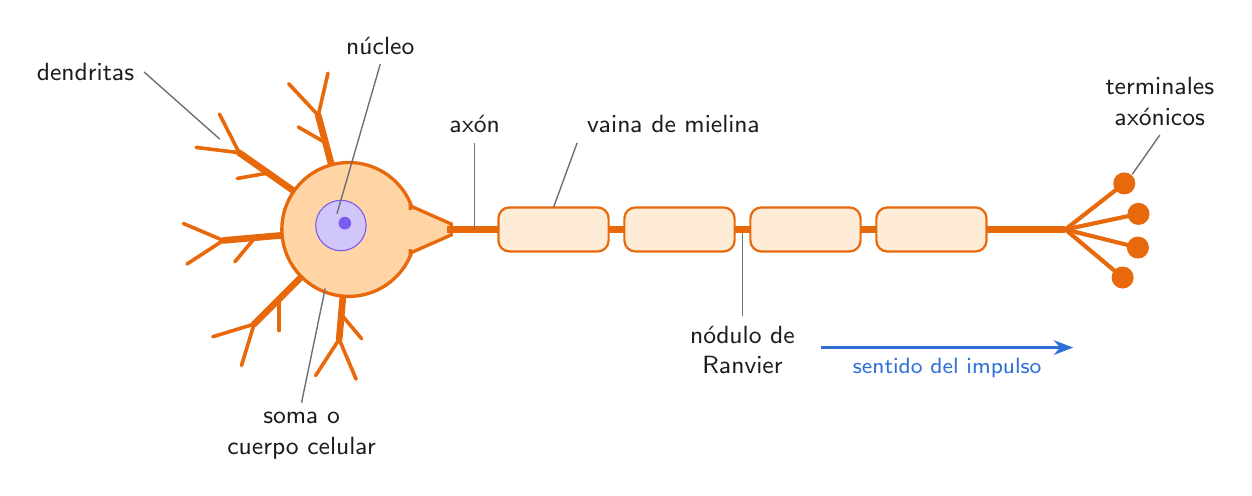
\begin{tikzpicture}[font=\small]
\neurona
\begin{scope}[gris,line width=0.5pt]
\draw (145:2.0) -- (-2.6,2.0) node[anchor=east,text=tinta] {dendritas};
\draw (-0.3,-0.75) -- (-0.6,-2.2) node[anchor=north,text=tinta,align=center] {soma o\\cuerpo celular};
\draw (-0.15,0.2) -- (0.4,2.1) node[anchor=south,text=tinta] {núcleo};
\draw (1.6,0) -- (1.6,1.1) node[anchor=south,text=tinta] {axón};
\draw (2.6,0.28) -- (2.9,1.1) node[anchor=south west,text=tinta] {vaina de mielina};
\draw (5.0,-0.05) -- (5.0,-1.1) node[anchor=north,text=tinta,align=center] {nódulo de\\Ranvier};
\draw (9.95,0.7) -- (10.3,1.2) node[anchor=south,text=tinta,align=center] {terminales\\axónicos};
\end{scope}
\draw[-{Stealth[length=7pt]},azul,very thick] (6.0,-1.5) -- (9.2,-1.5) node[midway,below,text=azul,font=\footnotesize] {sentido del impulso};
\end{tikzpicture}
\end{document}
